\chapter{Digital Calorimetry}
\label{sect:DECAL}

\section{Introduction}
As mentioned in \refsec{det:ecal}, several alternatives exist for the \ac{ECAL} design of \ac{ILD}. Here we present details of a proposed fully digital \ac{ECAL} that simply counts the number of pixels above threshold rather than measuring the energy deposited in each pixel which works based on the fact that the number of particles produced by an electromagnetic shower is proportional to the energy of the incident particle.

This approach has several potential benefits. Fundamentally it should allow for a slight improvement in the energy resolution as it is less senstive to fluctuations arising from landau fluctuations and varying path lengths as the particle traverses the active material. On top of this, the proposed technology choice will be to use highly granular ($\mathcal{O}$(50$\mu m$)) \ac{CMOS} \ac{MAPS}. This is the same technology as is used for the inner trackers and so this would allow a uniform technology solution across multiple detector components. It is also a much cheaper technology option than that used by the alternative \ac{ECAL} designs. The high granularity further allows for better pattern recognition with the calorimeter which can improve the performance of the particle flow algorithm applied in Pandora.

While the digital option provides these benefits it does come with one potential flaw referred to as saturation. In a digital calorimeter, if two particles pass through the same pixel, only one hit will be registered and so the total number of particles in the shower (and thus the energy of the shower) will be underestimated. The density of an EM shower scales according to the energy of the showering particle. As a result the rate of multiple occupancy in the pixels will increase with energy leading to a non linear relationship between a particles energy and the number of hits it generates within the detector. In practice this problem can be avoided by ensuring that the granularity of the detector is always greater than the density of the electromagnetic showers. For typical \ac{ILC} energies the density of the showers is estimated to be $\mathcal{O}$ 100 particles/mm$^2$ and so a granularity of at least 50$\times$50~$\mu$m$^2$ is required to ensure only one particle hits each pixel. Note that inn the analogue case this problem does not occur as the energy deposited in the pixel is what is measured and this will scale with the number of particles passing through the pixel.

\begin{figure}
  \centering
  \begin{subfigure}[t]{.45\textwidth}
    \centering
    
\includegraphics[width=1\linewidth,keepaspectratio]{DECALStudies/fig/cmos_3Tdesign}
  \end{subfigure}%%%
  \begin{subfigure}[t]{.45\textwidth}
    \centering
    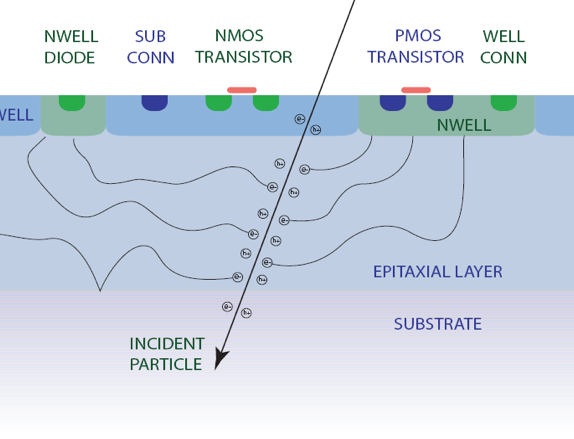
\includegraphics[width=1\linewidth,keepaspectratio]{DECALStudies/fig/nodeeppwell}
  \end{subfigure}
  \caption{Left: Schematic of the simplest layout for a \ac{CMOS} sensor using just three transistors. The first transistor, M$_{rst}$, acts as a switch to reset the charge collected at the diode. M$_{SF}$ allows the charge of the diode to be measured and amplified without removing the charge. Finally M$_{Sel}$ controls when the signal is read out from the pixel. Right: physical layout of a typical \ac{CMOS} pixel sensor.}
  \label{fig:cmosdesign}
\end{figure}

The requirement on the granularity is what ultimately leads to the decision to use a \ac{MAPS} based technology. For \ac{ILD}, using 50$\times$50~$\mu$m$^2$ pixels requires the use of ($\mathcal{O}$(10$^{12}$)) pixels. Having separate readout electronics, along with cooling and power supplies for each cell becomes impractical and porduces large dead space within the detector. By using \ac{MAPS} technology the electronics can instead be integrated into the silicon of the pixels leading to a more compact structure. \ac{CMOS} is then chosen as it is a cheap, well understood and commercial process for producing \ac{MAPS} structures. The typical layout of a \ac{CMOS} \ac{MAPS} pixel is shown in \reffig{fig:cmosdesign}. In practice this simple design is found to be unsatisfactory for use in particle physics due to the low signal yield due to parasitic losses to the PMOS transistor. A process referred to as INMAPS was developed at \ac{RAL}\cite{2008arXiv0807.2920B} which uses the addition of a deep p well around the PMOS transistor to mitigate the signal loss. The layout of this variation is shown in \reffig{fig:deeppwell}. Two sensors based on the deep p well design have already been produced (TPAC\cite{Ballin:2008rha} and CHERWELL\cite{MYLROIESMITH2013137}) and used to show the validity of this approach for producing a \ac{DECAL}\cite{Price:2013js}. In both cases the test pixels were based on a 50$\times$50~$\mu$m$^2$ design.


\begin{figure}
  \centering
  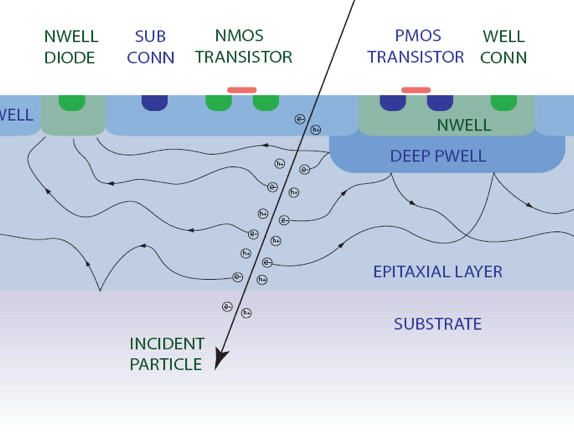
\includegraphics[width=0.5\textwidth,keepaspectratio]{DECALStudies/fig/deeppwell}
  \caption{\ac{CMOS} \ac{MAPS} sensor including deep p well implant to prevent parastic losses to the PMOS transistor\cite{MYLROIESMITH2013137}}
  \label{fig:deeppwell}
\end{figure}

Here we will present simulation studies looking at the optimization of the pixel dimensions for the sensors when including variation levels of realism such as noise, deadspace and clustering.  

\section{Event Generation and Detector Simulation}


Simulation of the \ac{DECAL} was performed in the GEANT4 based ILCSoft application, Mokka v08-05. The model used was based on an existing model for \ac{ILD}, ILD\_v01\_05, and so includes the high level of detail implemented for the\ac{ILD} letter of intent studies\cite{ILD} e.g. realistic geometries including support structures. The design was then adapated in three main ways. Firstly, the 300~$\mu$m thick active layer of silicon is divided into a thin active epitaxial layer (10-20~$\mu$m) and a deeper passive layer of silicon (280-290~$\mu$m.) The thin active layer represents what would be used in a typical \ac{CMOS} \ac{MAPS} sensor while the deeper passive layer is only included to prevent the need for changing the detailed layer structure of the exisiting model. In practice such a deep passive silicon layer would not be used. Secondly, the pixel pitch was reduced down to 5$\times$5~$\mu$m$^2$. This is smaller than can realistically be manufactured at present, however by using a narrow pixel pitch during the simulation the pixels can later be grouped together into larger virtual pixels with realistic dimensions preventing the need for simulating events at every pixel pitch required for the study and saves considerable processing time. The final change implemented was to remove the guard ring structures present in the analogue design. In the analogue design the guard rings are 1 mm metal rings placed around wafers of 18$\times$18 pixels. For the digital case these structures are not required and would result in a large amount of dead space in the detector due to the considerabley narrower pixel pitch. 

\begin{figure}
  \centering
  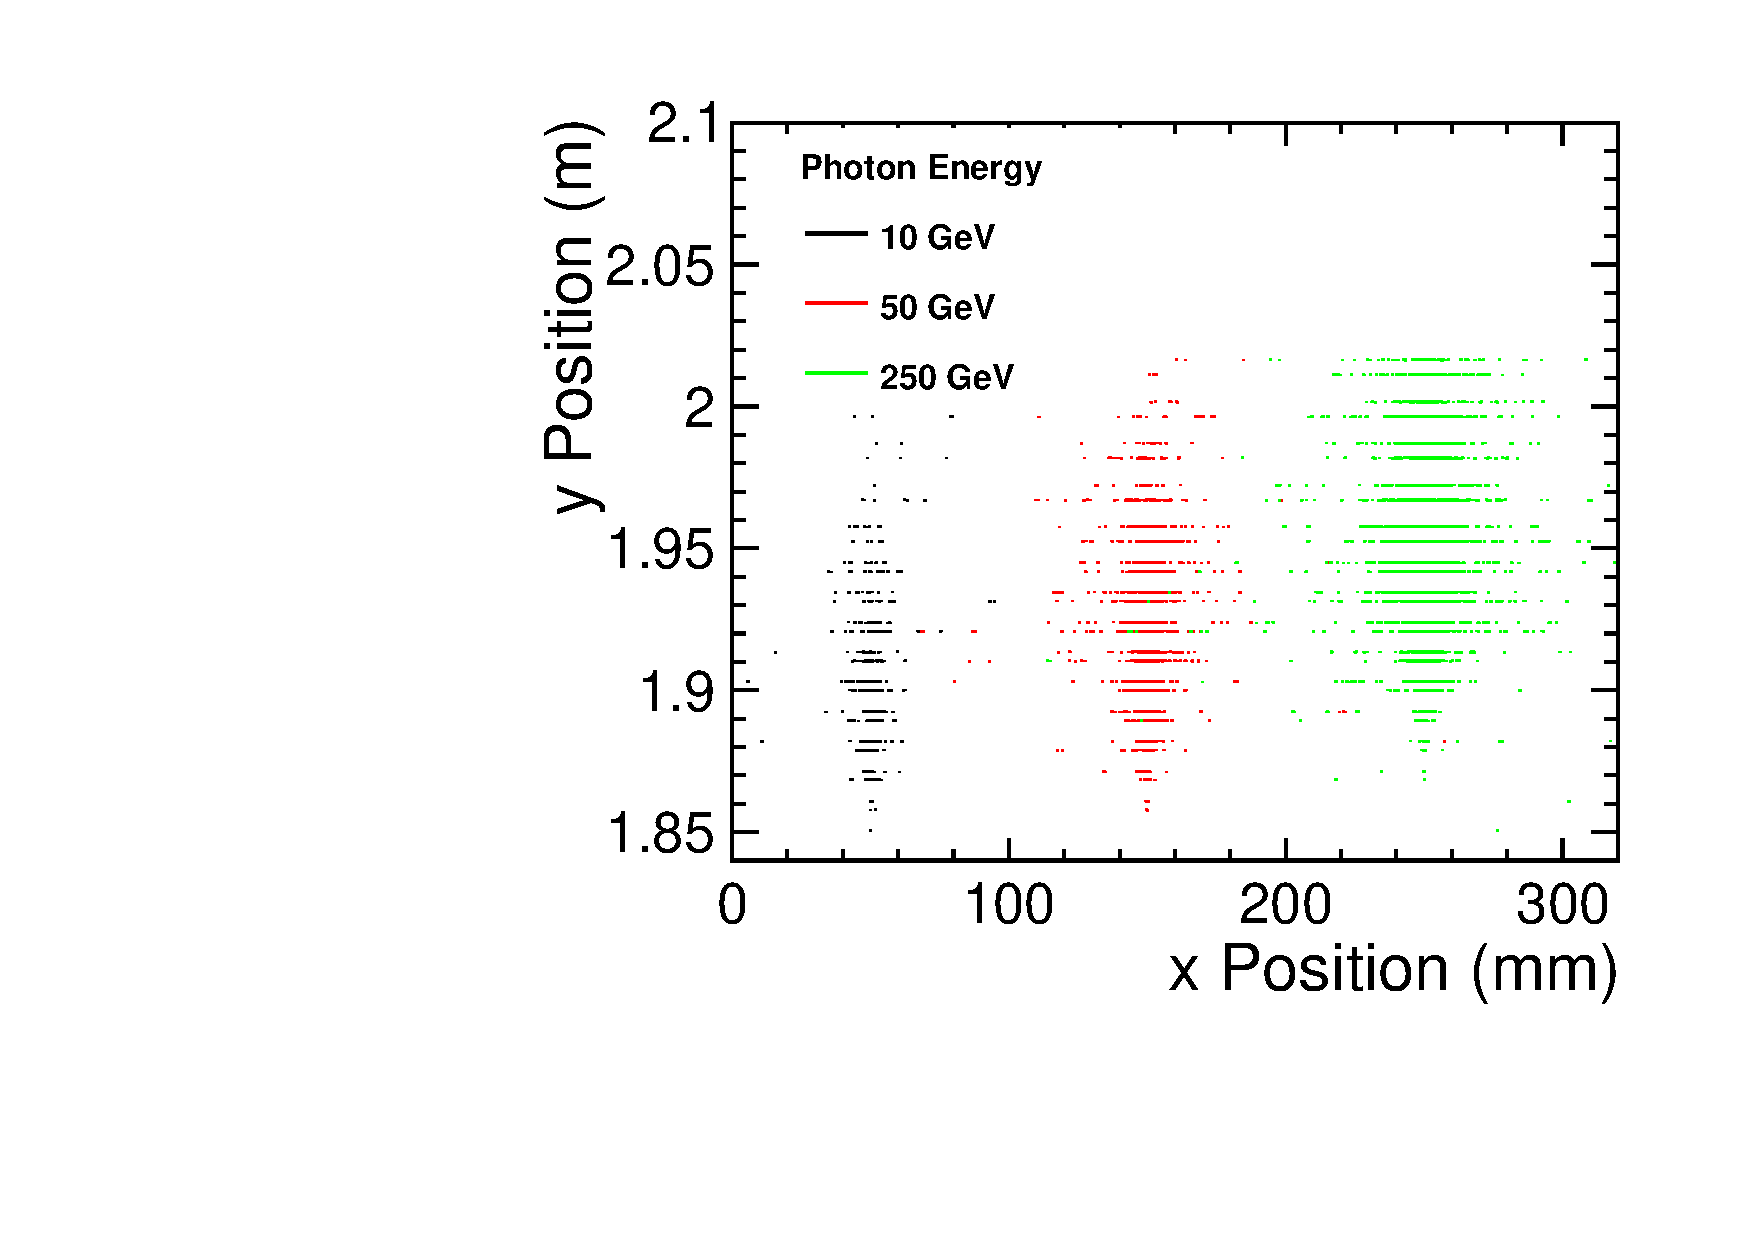
\includegraphics[width=0.7\textwidth,keepaspectratio]{DECALStudies/fig/ExampleEvents}
  \caption{Example of how EM showers look in the \ac{DECAL} for various photon energies. The y coordinate here represents the radial distance from the centre of the centre of the full detector.}
  \label{fig:exampleevents}
\end{figure}

Once the geometry was implemented, events were generated using the built in Mokka particle gun to fire photons through the \ac{ECAL}. When doing this the gun was placed immediately in front of the \ac{ECAL} to prevent showers forming earlier in the detector from interactions with the inner components such as the tracker. Photon were produced in 10 GeV intervals between 10 GeV and 100 GeV with an additional sample generated at 250 GeV representing the maximum energy possible at \ac{ILC}. For each energy, 10,000 events were generated to produce a large enough statistical sample to work with. Events were then generated using five different epitaxial thicknesses between 12 and 20 $\mu$m. In total this corresponds to a total of $\sim$ 500,000 events being generated. An example of what these events look like in the detector is shown in \reffig{fig:exampleevents}.

In order to be realistic, thresholds were applied on the energy deposited in a pixel as in practice this is always necessary to remove hits coming from electrical/thermal noise. The amount of energy deposited by a particle in a thin layer of material will typically follow a landau distribution. The threshold was chosen to be half of the most probable value (MPV) of the landau distribution to provide a balance between the amount of signal loss and potential background acceptance. The value of the MPV was found by fitting the energy ditributions measured in the simulation. For doing this, 10 GeV photons and 100$\times$100 $\mu$m$^2$ were used to prevent influence from saturation or from boundary effects where a particle deposits low amounts of energy from crossing the boundary across two pixels within one layer. As the amount of energy depsosited depends only on the epitaxial layer thickness and not the pixel pitch, the threshold was only evaluated for each epitaxial thickness then applied uniformly across all pitches. An example of one of the fits used is shown in \reffig{fig:thresholdfit}.

\begin{figure}
  \centering
  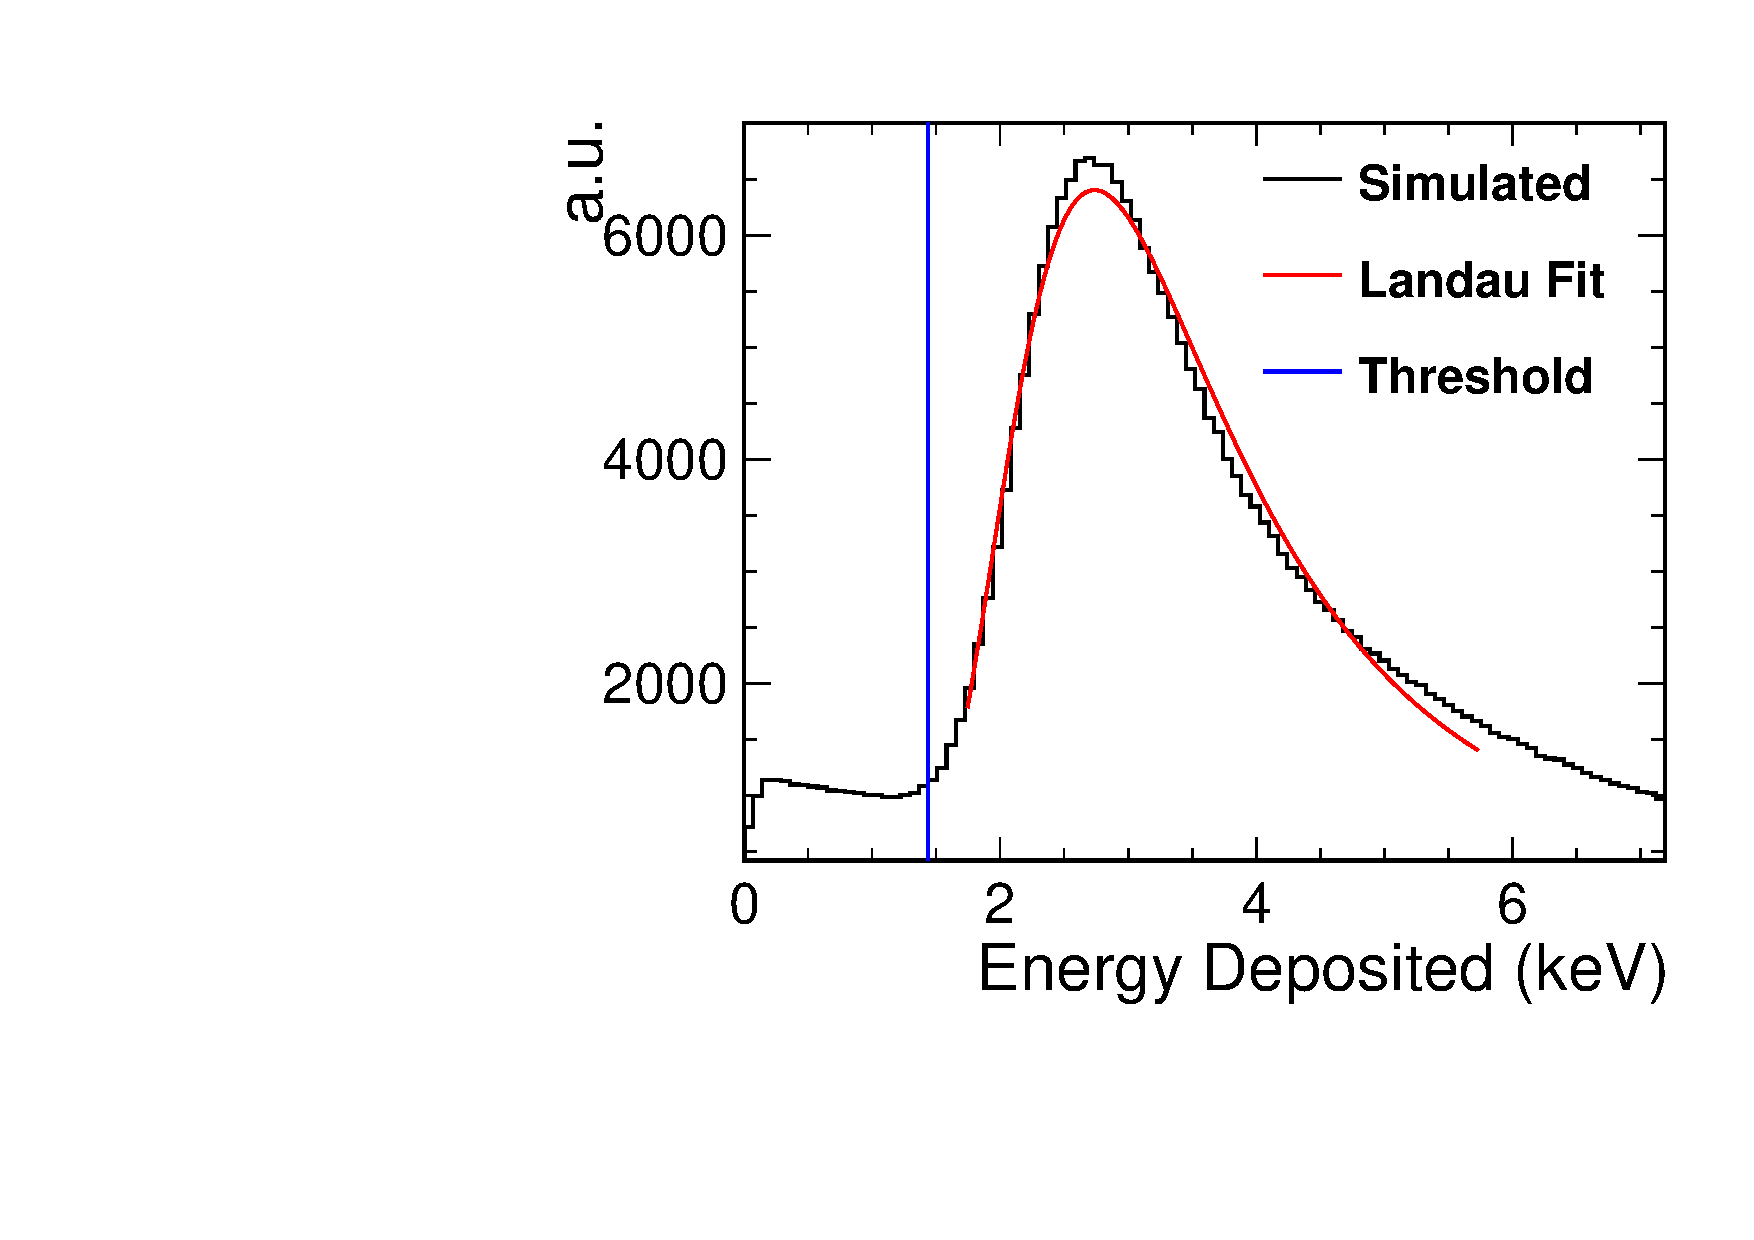
\includegraphics[width=0.7\textwidth,keepaspectratio]{DECALStudies/fig/Landau_100x12_10GeV.pdf}
  \caption{Energy deposited in a 100$\times$100 $\mu$m$^2$ pitch, 12$\mu$m thick pixel by a 10 GeV photon. The landau fit and resulting choice of threshold are also shown.}
  \label{fig:thresholdfit}
\end{figure}


\section{Pixel Design Optimization}

Ultimately the performance of any calorimeter is measured by the energy resolution, $\sigma_E/E$ , it can achieve. As such it is important to explain how this is defined for a digital calorimeter. Naively one could work on the basis that the energy of a particle is proportional to the number of particles produced in a shower and so define the resolution to be $\sigma_N/N$ where $N$ is the number of hits in the detector. While this is approximately true, it fails to account for the fact the number of particles produced in the shower may not be proportional to the number of hits due to multiple occupancies. A more reliable definition of the resolution has been found to come from first creating a calibration curve defining the relationship between the true energy of a particle, then using this curve to map back from the number of particles to a reconstructed energy for a particle. The energy resolution is then calculated by performing a gaussian fit to the reconstructed particle energies and defining the resolution to be $\sigma_{E,gaus}/E$. In the case that there is no saturation, this resolution should be equivalent to $\sigma_N/N$ as $N$ is linearly proportional to $E$. In all cases, the calibration curves are produced using one fifth of the statistical sample and the remaining four fifths are used to evaulate the energy resolution. Examples of how these calibration curves look for different pixel configurations are shown in \reffig{fig:calibrationcurves}. For wider pixels it is observed that the energy to hits relationship becomes non linear indicating detector saturation is occuring. 

\begin{figure}
  \centering
  
\includegraphics[width=0.7\textwidth,keepaspectratio]{DECALStudies/fig/dummy}
  \caption{Calibration curves describing the relationship between the number of pixel hits observed and the energy of the incident particle for various pixel configurations.}
  \label{fig:calibrationcurves}
\end{figure}

\begin{figure}
  \centering
  
\includegraphics[width=0.7\textwidth,keepaspectratio]{DECALStudies/fig/dummy}
  \caption{Gaussian fit to reconstructed energy for various pixel configurations.}
  \label{fig:gausfits}
\end{figure}

Having generated the calibration curves, the energy resolution was then evaluated for every photon energy and pixel configuration (see \reffig{fig:gausfits}). The performance for each pixel configuration is then evaluated by performing a second order polynomial fit to $\sigma_E/E$ vs 1/$\sqrt{E}$. This method allows the parameters a, b and c to be extracted in accordance with \refeq{eq:resolutionformula}, where a is the stochastic term, b is the noise term and c is the constant/leakage term. Typically the resolution of an \ac{ECAL} can be expected to be dominated by the stochastic term.

\begin{equation}
  \label{eq:resolutionformula}
  \frac{\sigma_E}{E}=\frac{a}{\sqrt{E}} \oplus \frac{b}{E} \oplus c
\end{equation}

The values of a, b and c for every pixel configuration are shown in \reffigs{fig:stochasticterm}, \ref{fig:noiseterm} and \ref{fig:constantterm}. One can see that the stochastic and noise terms dominate the overall resolution, however they show very different dependencies on the pixel configuration. The stochastic is seen to be lowest for wider pixel pitches whereas the noise term is lowest for the narrower pitches. One can trivially explain the distribution in the noise term as arising from saturation effects as for wider pixels the granularity of the detector will be less than the density of the EM showers. This results in a non linear response for the detector which gets translated into a non linear energy resolution and so a large second order term in the 1/$\sqrt{E}$ fit. Further evidence for this explanation can be seen in \reffig{fig:occupancy}.

\begin{figure}
  \centering
  
\includegraphics[width=0.7\textwidth,keepaspectratio]{DECALStudies/fig/dummy}
  \caption{Stochastic term of the energy resolution fits for all pixel configurations}
  \label{fig:stochasticterm}
\end{figure}
\begin{figure}
  \centering
  
\includegraphics[width=0.7\textwidth,keepaspectratio]{DECALStudies/fig/dummy}
  \caption{Noise term of the energy resolution fits for all pixel configurations}
  \label{fig:noiseterm}
\end{figure}
\begin{figure}
  \centering
  
\includegraphics[width=0.7\textwidth,keepaspectratio]{DECALStudies/fig/dummy}
  \caption{Constant term of the energy resolution fits for all pixel configurations}
  \label{fig:constantterm}
\end{figure}

\begin{figure}
  \centering
  
\includegraphics[width=0.7\textwidth,keepaspectratio]{DECALStudies/fig/dummy}
  \caption{Pixel occupancy for 250 GeV photons.}
  \label{fig:occupancy}
\end{figure}


To understand the stochastic term requires examination of the landau distributions as shown in \reffigs{fig:landaupitches} and \ref{fig:landauthickness}. One can see that as the aspect ratio decreases, a secondary peak appears in the energy deposition distribution at low energies. This is a result of particles crossing between pixels and so leaving only a fraction of the expected energy per layer in each pixel. The result of the boundary crossings is that there is a greater fluctuation on the number of pixels above threshold as rather than consistently observing one hit per particle per layer, it is possible to also get no hits if the deposits across both pixels are below threshold, or more likely an additional hit from both deposits being above threshold. 

\begin{figure}
  \centering
  
\includegraphics[width=0.7\textwidth,keepaspectratio]{DECALStudies/fig/dummy}
  \caption{Variation in the landau distributions for 10 GeV photons as a function of the pixel pitch.}
  \label{fig:landaupitches}
\end{figure}
\begin{figure}
  \centering
  
\includegraphics[width=0.7\textwidth,keepaspectratio]{DECALStudies/fig/dummy}
  \caption{Variation in the landau distributions for 10 GeV photons as a function of the epitaxial thickness.}
  \label{fig:landauthickness}
\end{figure}

In practice the optimal pixel configuration should provide a balance between the boundary crossing and multiple occupancy effects. Because the saturation level is a function of the incident particle energy, the optimal design will vary depending on the energy scale the detector is intended to study. For lower energy scales a wider pixel is optimal as the saturation is inherently low and the wide pitch will minimise boundary crossings. For higher energies the saturation rate will dominate and so a narrower pixel is preferred. In both cases a thinner pixel is preferred to minimise boundary crossings. The net resolutions observed at three different energy scales are shown in \reffigs{fig:resolution10}, \ref{fig:resolution50} and \ref{fig:resolution250}. The variation in the optimal configuration is seen to agree with that predicted from our boundary corssing and occupancy considerations.

\begin{figure}
  \centering
  
\includegraphics[width=0.7\textwidth,keepaspectratio]{DECALStudies/fig/dummy}
  \caption{Energy resolution for 10 GeV photons.}
  \label{fig:resolution10}
\end{figure}

\begin{figure}
  \centering
  
\includegraphics[width=0.7\textwidth,keepaspectratio]{DECALStudies/fig/dummy}
  \caption{Energy resolution for 50 GeV photons.}
  \label{fig:resolution50}
\end{figure}

\begin{figure}
  \centering
  
\includegraphics[width=0.7\textwidth,keepaspectratio]{DECALStudies/fig/dummy}
  \caption{Energy resolution for 250 GeV photons.}
  \label{fig:resolution250}
\end{figure}

\section{DigiMAPs}

While the above simulations highlight the dominant effects that must be considered in designing a digital calorimeter, they remain somewhat unrealistic. In particlur they lack effects such as charge collection efficiencies within the pixels, pixel noise and the effects of clustring algorithms. These effects are not possible to study within standard GEANT4 simulations, instead they are added in later using a package referred to as DigiMAPS(CITATION) developed by the \ac{CALICE} collaboration. This package takes the output hits from MOKKA, applies the effects of added levels of realism to remove/create new hits, then outputs an updated collection of hits for analysis. The effects that have been considered are listed below.

\begin{itemize}
\item Charge spread
\item Noise Effects
\item Clustering
\item Threshold spread
\end{itemize}

To understand how the effect these different factors have on the energy resolution, the energy resolution for a specific pixel configuration and photon energy (SPECIFY THESE) is plotted as a function of the threshold applied to the pixel after each additional level of realism is included.

\subsection{Pixel Design Optimization Revisited}

Now that these additional levels of realism have been included, it is important to evaluate the impact they have on the optimal pixel configuration. This is done using the exact same procedure. When applying DigiMAPS all effects except the charge spread are included. The resulting values for the stochastic, noise and constant terms are shown in \reffigs{fig:stochastictermDigi}, \ref{fig:noisetermDigi} and \ref{fig:constanttermDigi}.

\begin{figure}
  \centering
  
\includegraphics[width=0.7\textwidth,keepaspectratio]{DECALStudies/fig/dummy}
  \caption{Stochastic term of the energy resolution fits for all pixel configurations}
  \label{fig:stochastictermDigi}
\end{figure}
\begin{figure}
  \centering
  
\includegraphics[width=0.7\textwidth,keepaspectratio]{DECALStudies/fig/dummy}
  \caption{Noise term of the energy resolution fits for all pixel configurations}
  \label{fig:noisetermDigi}
\end{figure}
\begin{figure}
  \centering
  
\includegraphics[width=0.7\textwidth,keepaspectratio]{DECALStudies/fig/dummy}
  \caption{Constant term of the energy resolution fits for all pixel configurations}
  \label{fig:constanttermDigi}
\end{figure}


blah blah, describe changes seen from before digimaps was applied

\begin{figure}
  \centering
  
\includegraphics[width=0.7\textwidth,keepaspectratio]{DECALStudies/fig/dummy}
  \caption{Energy resolution for XXX GeV photons.}
  \label{fig:resolutionXXXDigi}
\end{figure}

For the typical energy scale for the \ac{ILC} (100 GeV), the optimal pixel configuration is found to be at BLAH BLAH as shown in \reffig{fig:resolutionXXXDigi}. The resulting resolution is given by:

\begin{equation}
  \frac{\sigma_E}{E}=\frac{XX\%}{\sqrt{E}} \oplus \frac{XX\%}{E} \oplus XX\%
\end{equation}



\section{Conclusion}
